\clearpage

\section{Oxford Nanopore: cDNA Sequencing}
%https://www.nature.com/articles/s41587-020-0731-9

\subsection{Introduction}
Shortly following the revolutionary success of PacBio's SMRT to generate significantly longer reads in real-time (reviewed in \cref{tab: longread_isoseqstudies}), Oxford Nanopore Technologies (ONT) introduced another long-read, single-molecule sequencing technology with the commercial release of the MinION in 2014. In contrast to all other major sequencing applications including PacBio's SMRT sequencing which relies on "sequencing-by-synthesis" approach, ONT technology pioneered the novel approach of nucleic acid sequencing using protein nanopores for direct inference of the sequence (\cref{fig:ONT_Mechanism}\textbf{a}); it is the only technology to directly read a single DNA strand rather than by measuring incorporation events on the template strand\cite{Jain2015}. Partly owing to the relatively lower cost and portability of ONT technology, nanopore sequencing has been widely used for transcriptome profiling (reviewed in \cref{tab: longread_ontstudies}), 
with theoretically no upper limit \cite{Loman2015} (the longest read to date is over 150kb), and with no bias towards length or GC content \cite{Oikonomopoulos2016, Weirather2017}.


\subsubsection{Mechanism}
The MinION is a hand-held portable USB-powered device. At its centre is a flow cell that contains a sensor array, which houses a total of 2048 individual nanopores that are controlled in four groups of 512 channels (allowing up to 512 independent DNA molecules to be sequenced simultaneously)\cite{Jain2015}. As an electric current is applied across the nanopore, the single-stranded DNA molecules translocates through the nanopore and subsequently interrupts the current in a nucleotide-dependent manner, thereby generating a unique signal of electric current perturbations as proxy of the underlying nucleotide sequence (\cref{fig:ONT_Mechanism}\textbf{a}). 

Successful nanopore sequencing requires the efficient capture and threading of single strand DNA into the pore, followed by the ability to identify individual DNA bases in a time-resolved manner. This was achieved through several key innovations\cite{Bayley2015}: 
\begin{enumerate}
	\item Generation of an internal positive charge within the protein nanopore to induce capture of negatively-charged DNA. Each nanopore is embedded into an electrical resistant membrane that is immersed in an electrolyte solution.
	\item Discovery and usage of biological pore proteins, from the \textit{α}HL\cite{N2005}, to the MspA from \textit{Mycobacterium smegmatis}\cite{Manrao2011}, and currently, the CsgG from E.coli. The modified CsgG pore contains a short and narrow channel constriction site, enabling distinct ionic currents at a single-nucleotide resolution. 
	\item Ratcheting the DNA through the pore for time-resolved base identification to discriminate individual nucleotide signals from noisy background with a processive enzyme (motor protein, \cref{fig:ONT_Mechanism}\textbf{a,b}), which controls DNA movement and reduces the translocation speed of the molecule (average speed of 450bp/s) for improved signal\cite{Rang2018}. This processive enzyme is ligated to 5'end of both strands during library preparation.   
\end{enumerate}

\begin{figure}[]
	\centering
	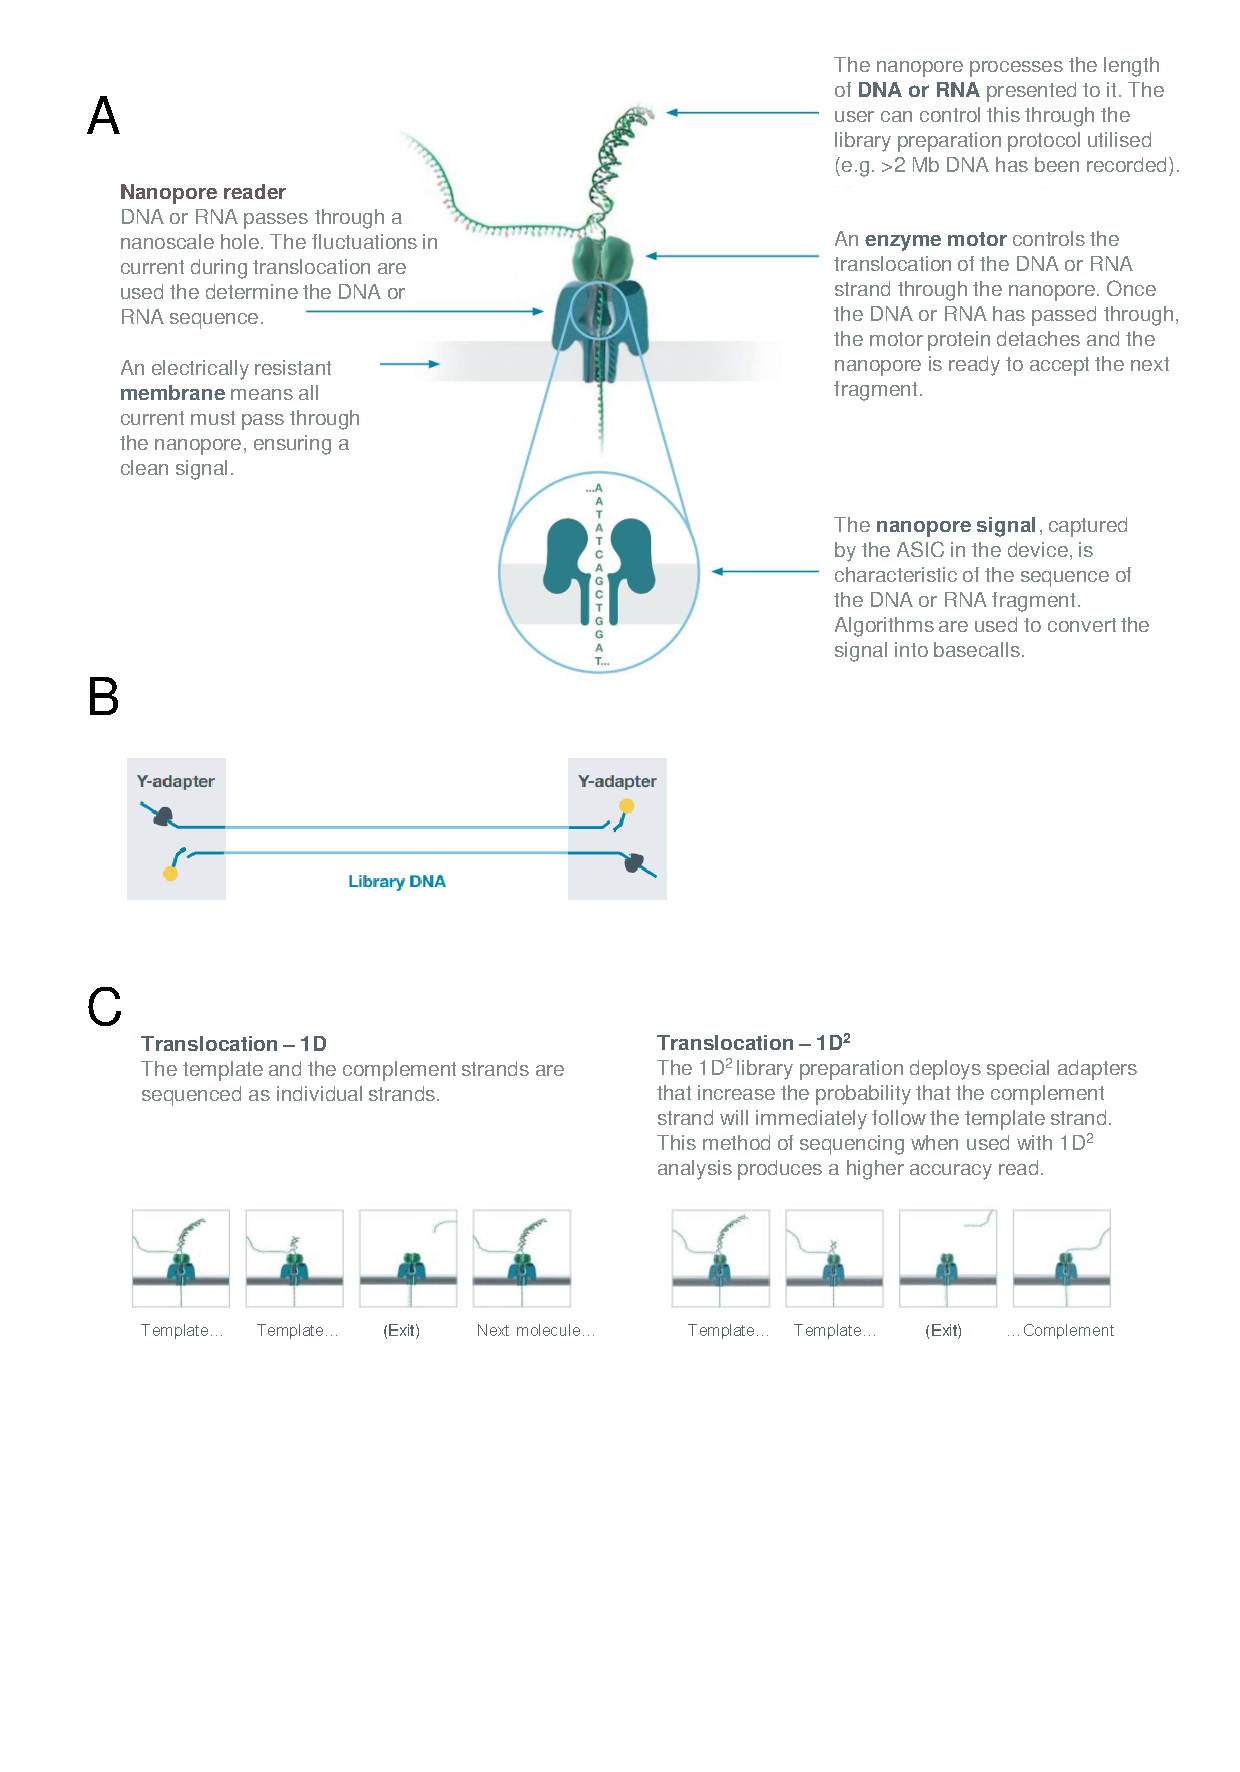
\includegraphics[page=1,trim={0 6cm 0 0 },clip, scale = 0.8]{Figures/ProjectDevelopment_FiguresONT}
	\captionsetup{width=0.95\textwidth}
	\caption[Oxford Nanopore Sequencing]%
	{\textbf{Oxford Nanopore Sequencing}: \textbf{a)} Oxford Nanopore Technologies pioneered the development of sequencing DNA through a biological nanopore. The translocation of the sequence, controlled by the enzyme motor protein, causes nucleotide-sensitive perturbations in the electric current. \textbf{b)} The structure of the library DNA with ligation of the sequencing adapter, containing the motor protein (brown circle), to both template and complementary strands. \textbf{c)} Two sequencing translocation modes are currently offered, generating either 1D or 1D\textsuperscript{2} reads. Figures are taken from Oxford Nanopore Product Brochure July 2018.}
	\label{fig:ONT_Mechanism}
\end{figure}

\vspace{1cm}
% https://community.nanoporetech.com/posts/flo-minxxx-x-rx-x-r
\subsubsection{Performance and Run Quality Metric}
One major limitation of nanopore sequencing is the relatively high error rate compared to short-read technologies, which can arise from error during sequencing or from translating the raw electric signal into a DNA sequence (basecalling)\cite{Rang2018}. The first error is exacerbated by the fact that several nucleotides occupy the pore at any given time point, resulting in multiple influences, and that the signal does change with translocation of homopolymers. However over recent years, major advances in both the basecalling algorithms, the chemistry and nanopore itself has drastically increased the initial accuracy from 60\% \cite{Jain2015} to 98.3\% (vR.9.4.1 and Bonito) (\cref{fig:ONT_advances}). This includes the improved chemistry to sequence both the template and the complementary strand immediately after, thereby attaining a more accurate consensus read (1D\textsuperscript{2}) that increases the accuracy of template reads (1D) alone by 5\%\cite{Rang2018} (\cref{fig:ONT_Mechanism}\textbf{c}), though at the expense of throughput \cite{NanoporeCommunityPosts}. Of note, earlier releases of nanopore sequencing offered 2D sequencing which involved ligation of both strands with a hairpin adapter, though this has been largely replaced by (1D\textsuperscript{2}) sequencing. However, the error rate still falls short of 99\% offered by PacBio's CCS reads and short-read platforms, and errors near splice sites can result in spurious alignments and in correct clustering of reads. Other approaches to mimic the PacBio's circular consensus approach and generate circularised templates for nanopore sequencing have been proposed (INC-seq \cite{Li2016c} and R2C2 \cite{Volden2018}), with accuracy approaching 97.5\%. However, such methods are laborious and are not commonly used.  

\begin{figure}[h]
	\centering
	\includegraphics[page=2,trim={0 19cm 0 0 },clip, scale = 0.8]{Figures/ProjectDevelopment_FiguresONT}
	\captionsetup{width=0.95\textwidth}
	\caption[Significant advances in Oxford nanopore sequencing read accuracy]%
	{\textbf{Significant advances in Oxford nanopore sequencing read accuracy}: Optimisation in the structure of nanopores (chemistry updates) and development in basecalling algorithms have led to drastic improvements in read accuracy. The R7 and R9 nanopore series is based on the MspA and CsgG protein respectively. Of note, the figure does not include the latest chemistry (1D\textsuperscript{2}) or nanopore development (R.10.4, this involves a longer barrel and two pinch points to provide better resolution of homo-polymer sequences). Figure is taken from Rang et al.(2018)\cite{Rang2018}}
	\label{fig:ONT_advances}
\end{figure}

\newpage
In contrast to Iso-Seq Sequel, real-time feedback of the nanopore sequencing progress is obtained from MinION with information provided on the run statistics (i.e. the total number of reads generated so far) and a summary of the channel states over time (duty time plot). The channel state is an indication of the pore occupancy and is classified as either i) Sequencing (active with current DNA translocation), ii) Pore (active but without DNA translocation), iii) Recovering, iv) Inactive and v) Unclassified - channels are divided into 4 groups and used sequentially to maximise throughput, and unclassified channels are those not currently used. The duty time plot provides a good assessment of the current performance of the run, and an early indication whether to continue or stop the run (examples of successful and suboptimal runs are depicted in \cref{fig:ONTPoreOccupancy}). 

\begin{figure}[]
	\centering
	\includegraphics[page=6,trim={0 14cm 0 0 },clip, scale = 0.8]{Figures/ProjectDevelopment_FiguresONT}
	\captionsetup{width=0.95\textwidth}
	\caption[Examples of successful and suboptimal ONT nanopore sequencing runs]%
	{\textbf{Examples of successful and suboptimal ONT nanopore sequencing runs}: Shown are duty time plots from \textbf{a)} Good quality run, which is determined by the majority of pores in the "Sequencing" state (bright green), \textbf{b)} Suboptimal run with channels being blocked, as indicated by an accumulation of pores in the "Recovering" state (dark blue), \textbf{c)} Suboptimal run with low pore occupancy, indicated by the high ratio of "Pore" (dark green) to "Sequencing" state, and \textbf{d)} Suboptimal run with flow cell failure with the majority of pores in "Inactive state" (light blue). Channel blocking typically occurs when there are contaminants in the library. Conversely, low pore occupancy suggests insufficient loading material or poor library preparation (poor ligation reaction). Flow cell failure indicate damaged channel or membranes, which can be caused by multiple factors (air bubbles, osmotic imbalance, presence of detergents in library). Figures are taken from WTAC material. Channel states are classified as sequencing (bright green), pore (dark green), recovering (dark blue), inactive (light blue) and unclassified (grey).}
	\label{fig:ONTPoreOccupancy}
\end{figure}

\clearpage
\subsection{Lab Workflow}
\label{chap:ont_labpipeline}
This section describes the library preparation for ONT cDNA sequencing used in this thesis. At the time I was performing nanopore sequencing, the ONT was less advanced that the PacBio with less detailed protocols. Nanopore sequencing was therefore conducted on a subset of samples as a source of validation and technology comparison. For a fairer and more direct comparison, all steps prior to the ONT library preparation were adopted from the Iso-Seq protocol, including conversion of RNA to cDNA using the SMARTer PCR cDNA synthesis (ClonTech) (described in \cref{section:ch2_cDNA_synthesis_explanation}) and large scale DNA amplification using the GXL DNA Polymerase (workflow is depicted in \cref{fig:ONT_WholeProtocol}). Targeted profiling of the transcriptome using nanopore sequencing was performed by conducting ONT library preparation on the same samples after cDNA synthesis, amplification and target enrichment with IDT (described in \cref{section:ch2_targetcapture_explanation}) (workflow is depicted in \cref{fig:ONT_TargetedProtocol}). The nanopore reads thus have the same cDNA primers and barcode sequences as the Iso-Seq reads (refer to \cref{tab:barcode_primers} for sequences).   

Post cDNA synthesis and amplification, ONT library preparation is similar to the Iso-Seq library preparation  (described in \cref{chap:isoseq_labpipeline}) in that cDNA molecules are repaired for ends, and then ligated with adapters (outlined in \cref{fig:ONT_WholeProtocol}). The only difference is the nature of the adapters - the polymerase is loaded after adapter ligation in PacBio, whereas the motor enzyme is already pre-bound to the adapters in ONT. 

\begin{figure}[]
	\centering
	\includegraphics[page=4,trim={0 6cm 0 0 },clip, scale = 0.7]{Figures/ProjectDevelopment_FiguresONT}
	\captionsetup{width=0.95\textwidth}
	\caption[ONT Global Transcriptome Profiling Lab Workflow]%
	{\textbf{ONT Global Transcriptome Profiling Lab Workflow}: For a fair and direct comparison of technology, the first part of the lab workflow for the global transcriptome profiling using nanopore sequencing was identical as that for the PacBio Iso-Seq. RNA was converted to cDNA using SMARTer PCR cDNA synthesis (ClonTech) and amplified to two reactions in order to sufficient material downstream. Amplified DNA was then split and purified using the 1x and 0.4x AMPure beads for Iso-Seq, and 0.9x for ONT. Equimolar amounts of purified DNA was then used for respective library preparation, before sequencing on the PacBio Sequel and ONT MinION.}
	\label{fig:ONT_WholeProtocol}
\end{figure}

\begin{figure}[]
	\centering
	\includegraphics[page=5,trim={0 11cm 0 0 },clip, scale = 0.7]{Figures/ProjectDevelopment_FiguresONT}
	\captionsetup{width=0.95\textwidth}
	\caption[ONT Targeted Transcriptome Profiling Lab Workflow]%
	{\textbf{ONT Targeted Transcriptome Profiling Lab Workflow}: For a fair and direct comparison, targeted transcriptome profiling was similarly performed on the same samples that had been prepared for Iso-Seq transcriptome profiling. RNA was barcoded and similarly converted to cDNA using SMARTer PCR cDNA synthesis kit. Amplified cDNA was then enriched for target genes using IDT Target Capture and subjected to respective library preparation. Of note, this workflow is identical to the global transcriptome profiling workflow depicted in \cref{fig:ONT_WholeProtocol} with the exception of using barcodes for cDNA synthesis (boxed green) and the additional step of target enrichment (boxed orange)}
	\label{fig:ONT_TargetedProtocol}
\end{figure}


\subsubsection{ONT MinION Library Preparation}
\label{sec: ONTlib_preparation}
After obtaining high-quality and full-length cDNA, nanopore library preparation was proceeded with 1D sequencing by ligation protocol (SQK-LSK109, \cref{fig:ONT_Protocol}) to generate 1D reads (\cref{fig:ONT_Mechanism}\textbf{c}). The library preparation was simple: cDNA ends were repaired and dA-tailed using the NEBNext End Repair/dA-tailing Module. Following 1x AMPure Bead Purification of cDNA end-repaired products, ONT sequencing adapters were then ligated onto the 5' prepared ends and subjected to another round of 0.4x AMPure Bead Purification. The library was then ready for loading onto the MinION. The ONT sequencing adapters (depicted in \cref{fig:ONT_Mechanism}\textbf{b}) contained a dT overhang for ligation to the dA-ends of cDNA, the pre-bound motor protein, and a cholesterol moiety which facilitates DNA capture by tethering and restricting the DNA molecule to the flow cell's lipid membrane.

\subsubsection{Priming the Flow Cell and Sequencing}
Nanopore sequencing was performed on the MinION using a Min106D Flow cell (contains the R9 nanopore shown in \cref{fig:ONT_advances}). Prior to sequencing, the flow cells were tested for the total number of functional pores present and only used if more than 800 pores were available, as recommended by ONT. The flow cell was then primed for sequencing with a "Running buffer with fuel mix" (RBF), which contained the substrate cofactor essential for efficient motor protein activity (i.e. ATP for the ATPase activity of the helicase component of the translocation motor). The library was then loaded into the MinION with Library Loading Beads (LLB) - these are sepharose beads that work similarly to Iso-Seq MagBeads by immobilising the library to the lipid membrane, which is then tethered together with the cholesterol moiety.    

\begin{figure}[]
	\centering
	\includegraphics[page=3,trim={0 16cm 0 0 },clip, scale = 0.7]{Figures/ProjectDevelopment_FiguresONT}
	\captionsetup{width=0.95\textwidth}
	\caption[ONT library preparation with ligation sequencing kit]%
	{\textbf{ONT library preparation with ligation sequencing kit}: High-quality and full-length cDNA was proceeded with ONT's ligation sequencing kit (SQK-LSK109), which involved repairing ends and dA-tailing followed by ligation of the ONT sequencing adaptors. The motor protein and cholesterol moiety are represented by the brown and yellow circle respectively. Figure is adapted from ONT Nanopore Protocol 1D amplicon/cDNA by Ligation (SQK-LSK109)}
	\label{fig:ONT_Protocol}
\end{figure}

 

\clearpage
\subsection{Bioinformatics Pipeline}
This section describes the bioinformatic pipeline that was used to process ONT cDNA sequencing data generated using the whole transcriptome (n = 2) in \cref{ch: whole_transcriptome} and targeted transcriptome approach (n = 20) \cref{ch: targeted_transcriptome}. 

Unlike the Iso-Seq bioinformatics pipeline which was largely established by PacBio (described in \cref{section:isoseq_bioinformatics}, \cref{fig:isoseq_bioinformatics_Pipeline}), the bioinformatics pipeline for processing ONT raw reads was less defined and streamlined. While significant improvements in bioinformatic tools have been released by ONT over the last 2 years, many of the new tools were only applicable to sequencing data generated from ONT-specific protocols and primers. Consequently, given that ONT sequencing data in this thesis was generated using the same primers and barcodes as Iso-Seq sequencing data for a fairer comparison, the initial stage of the bioinformatics pipeline was adapted from the Wellcome Trust Advanced Course: RNA Transcriptomics (2018), provided by J.Ragoussis (referred as WTAC), and refined using ERCC as benchmark. Many of the downstream tools developed for Iso-Seq were then similarly applied for the latter stage of ONT bioinformatics pipeline, bar the substitution of \textit{TAMA} for \textit{Cupcake} for transcript collapse (\cref{fig:ONT_PacBio_bioinformatics}). 

The steps for processing sequencing data from the whole and targeted transcriptome approach is largely similar, with the exception of an additional step of barcode demultiplexing in the targeted approach as 10 samples were barcoded and sequenced simultaneously in one flow cell (\cref{fig:ONT_Targeted_bioinformatics}). 

\begingroup
\parindent=0em
\etocsettocstyle{\rule{\linewidth}{\tocrulewidth}\vskip0.5\baselineskip}{\rule{\linewidth}{\tocrulewidth}}
\etocsetnexttocdepth{5}
\localtableofcontents 
\endgroup

\begin{figure}[htp]
	\centering
	\includegraphics[page=15,trim={0cm 6cm 0cm 0cm},clip,scale = 0.8]{Figures/ProjectDevelopment_Figures}
	\captionsetup{width=0.95\textwidth,singlelinecheck=off}
	\caption[Comparison of bioinformatics pipeline for processing PacBio Iso-Seq and ONT 1D-reads]%
	{\textbf{Comparison of bioinformatics pipeline for processing PacBio Iso-Seq and ONT 1D-reads}. Shown is a side-by-side comparison of the bioinformatics pipeline used to process PacBio Iso-Seq and ONT 1D-reads from initial processing of raw reads, alignment to reference genome with \textit{Minimap2}, collapse of reads to transcripts followed by annotation with \textit{SQANTI}. The bioinformatic pipelines adopted are largely similar between Iso-Seq and ONT with the difference primarily in the initial processing of raw reads; raw Iso-Seq reads were processed with \textit{Iso-Seq3} tool (PacBio) whereas raw ONT reads were processed with various community-based packages.   
	}
	\label{fig:ONT_PacBio_bioinformatics}
\end{figure}

\begin{figure}[htp]
	\centering
	\includegraphics[page=16,trim={0cm 6cm 0cm 0cm},clip,scale = 0.8]{Figures/ProjectDevelopment_Figures}
	\captionsetup{width=0.95\textwidth,singlelinecheck=off}
	\caption[Bioinformatics Pipeline for ONT Targeted Transcriptome]%
	{\textbf{Bioinformatics Pipeline for ONT Targeted Transcriptome}. Shown is a detailed bioinformatics pipeline for processing ONT reads 1D reads from the targeted transcriptome, whereby 20 samples were barcoded and sequenced simultaneously on two flow cells (referred as Batch 2 and Batch 3 of the original Iso-Seq Targeted Transcriptome set). Supplementing \cref{fig:ONT_PacBio_bioinformatics}, raw ONT reads from each flow cell were processed and the demultiplexed into the respective samples, which were then processed independently for collapse and transcript quantification. All the samples from both batches were then merged into one complete dataset, while retaining sample-specific transcript expression. 
	}
	\label{fig:ONT_Targeted_bioinformatics}
\end{figure}


\subsubsection{Quality Control of Run, Base-calling and Filtering of Base-called Reads}
The performance of a Nanopore sequencing run was assessed using \textit{PycoQC}\cite{Leger2019} and the official Nanopore QC tutorial\cite{ONT2019NanoporeQC}, by evaluating the number of active pores during the run, the number of reads generated over time, and the length and quality score distribution of basecalled reads. A suboptimal run would be indicated by a low sequencing yield (<20kb), whereby the vast majority of pores were inactive or there was significant increase in the number of inactive pores over time. 

Raw reads were basecalled using \textit{Guppy}, a basecaller program which converts ONT's raw electrical signal to DNA sequence. Basecalling is a rapidly advancing field current basecallers developed by using neural networks and training machine-learning algorithms on real data\cite{Wick2019}. The latest released basecaller by ONT, Guppy has been shown to perform superior to other available basecallers with higher read accuracy and faster basecalling\cite{Wick2019}. Basecalled reads with read quality score < 7 (nanopore default passed quality) were then removed using \textit{Nanofilt}\cite{DeCoster2018} with default parameters. 

\subsubsection{Removing of Nanopore and cDNA sequencing adapters}
Similarly to the Iso-Seq bioinformatics pipeline, cDNA sequencing primer sequences and nanopore ligation adaptors were removed to prevent spurious alignment, using \textit{Porechop}\cite{Wick2017} (v0.2.4, parameters: --end\_size 100, --adapter\_threshold 90, --end\_threshold 75, --min\_trim\_size 15, --discard\_middle, --extra\_end\_trim 1). Under those parameters, a window of 100 nucleotides from each end of the reads were searched for a set of adaptors, which must have a minimum 90\% identity to be considered present for trimming and a minimum 75\% at the end of the reads; alignments smaller than 15bp or found within the middle of the reads (considered chimeric) were removed. By manually defining a unique set of adaptors that includes the cDNA primers (from Clontech SMARTer PCR cDNA synthesis kit), the ONT adaptors and corresponding polyA/T tail, it was possible to differentiate the strand orientation (\cref{fig:ONT_cdnatemplate}); the adapter sequences used for whole transcriptome and targeted transcriptome approach are given in \cref{fig:ONT_cdnatemplate}\textbf{b} and \cref{tab:ont_barcode} respectively. Sample demultiplexing in the targeted transcriptome approach was performed by including the 16bp barcode sequence; of note, the barcode is only present in the 3'end of the plus strand and 5'end of the minus strand, as part of the oligo-dT primer during cDNA synthesis (\cref{tab:barcode_primers}). Reads were therefore assigned to the sample with the highest identity at the 5'end and 3'end for the plus and minus strand respectively. 

\textit{Porechop} has been officially unsupported since 2018 and has been largely replaced by ONT's officially recommended tool, \textit{Pychopper}\cite{OxfordNanoporePychopper}. While \textit{Pychopper} is useful for ONT-specific barcode demultiplexing, it was not able to differentiate and orient reads from the plus and minus strand without unique sequences. Given that the ONT cDNA reads were generated using the SMARTer cDNA synthesis kit (Clontech) (described in \cref{section:ch2_cDNA_synthesis_explanation}), 5’ end of the plus and minus strands are reverse complements of each other with the only difference being that the plus strand ends with ATGGG and the minus strand ends with polyT (\cref{fig:ONT_cdnatemplate}). 

Trimmed reads with adaptors present at both ends were retained, and reads corresponding to the minus strand were reverse complemented. Using \textit{Cutadapt}\cite{Martin2011} (v2.9, -a "A{40}"), the polyA sequence was then trimmed 40 nucleotides from the 3'end.



\begin{figure}[ht]
	\begin{center}
		\includegraphics[page=7,trim={0cm 17cm 0cm 1cm},clip, scale = 0.7]{Figures/ProjectDevelopment_Figures.pdf}
	\end{center}
	\captionsetup{width=0.95\textwidth}
	\caption[Structure of ONT library cDNA template]%
	{\textbf{Structure of ONT library cDNA template}: Shown is the \textbf{a)} final structure of cDNA molecules for ONT sequencing, after cDNA synthesis and adaptor ligation, and the corresponding differentiating start and end sequence for the plus and minus strands \textbf{b)} without and \textbf{c)} with barcodes. The original cDNA molecules are outlined in purple and green, and the ONT boxes indicate the position of the ONT adaptors. In cases where multiplexing is performed, the barcode location is indicated in red (see \cref{tab:barcode_primers} and \cref{tab:ont_barcode} for barcode sequences). Of note, only the plus strand end sequence and the minus strand start sequence contain the barcode and are used for sample demultiplexing, whereas the plus strand start and minus strand end sequence are identical across all barcoded samples. The brown and orange circle refer to the motor protein and cholesterol moiety respectively. The start and end of the strand is defined by the 5' and 3' end respectively. }
	\label{fig:ONT_cdnatemplate}
\end{figure}

\begin{landscape}
	\begin{table}[]
		\centering
		\begin{tabular}{@{}ccccc@{}}
			\toprule
			\multirow{2}{*}{Barcoded  Samples} & \multicolumn{2}{c}{Plus strand} & \multicolumn{2}{c}{Minus strand} \\ \cmidrule(l){2-5} 
			& Start sequence & End sequence & Start sequence & End sequence \\ \midrule
			BC1 & \multirow{10}{*}{\begin{tabular}[c]{@{}c@{}}TTGCTAAG\\ CAGTGGTA\\ TCAACGCA\\ GAGTACAT\\ GGG\end{tabular}} & AAAAAACGCACTCTGATATGTGGCA & CACATATCAGAGTGCGTTTTTT & \multirow{10}{*}{\begin{tabular}[c]{@{}c@{}}CCCATGTAC\\ TCTGCGTTG\\ ATACCACT\\ GCTTAGCAAT\\ ACGTAACT\end{tabular}} \\
			BC2 &  & AAAAAAACTCACAGTCTGTGTGTGCA & ACACACAGACTGTGAGTTTTTTT &  \\
			BC3 &  & AAAAAAACTCTCACGAGATGTGTGCA & ACACATCTCGTGAGAGTTTTTTT &  \\
			BC4 &  & AAAAAAACGCGCGTGTGTGCGTGGCA & CACGCACACACGCGCGTTTTTTT &  \\
			BC5 &  & AAAAAAAACGCGAGAGTCGAGTGGCA & CACTCGACTCTCGCGTTTTTTTT &  \\
			BC6 &  & AAAAAAAACAGCTGATATATATGGCA & CATATATATCAGCTGTTTTTTTT &  \\
			BC7 &  & AAAAAAACACATAGAGATACAGAGCA & TCTGTATCTCTATGTGTTTTTTT &  \\
			BC8 &  & AAAAAAACGCAGCGCTCGACTGTGCA & ACAGTCGAGCGCTGCGTTTTTTT &  \\
			BC9 &  & AAAAAAATCTGTCTCGCGTGTGTGCA & ACACACGCGAGACAGATTTTTTT &  \\
			BC10 &  & AAAAAAACTCTGAGATAGCGCGTGCA & ACGCGCTATCTCAGAGTTTTTTT & 
		\end{tabular}
		\captionsetup{width=0.9\linewidth}
		\caption[ONT adapter sequences for plus and minus strand of barcoded samples]%
		{\textbf{ONT adapter sequences for plus and minus strand of barcoded samples}. Tabulated are the sequences used in \textit{Porechop} for sample demultiplexing and identifying the plus and minus strands. As depicted in \cref{fig:ONT_cdnatemplate}, only the plus strand end sequences and the minus strand start sequences contain the sample-specific barcode sequence (reverse complementary of one another). BC - Barcode}
		\label{tab:ont_barcode}
	\end{table}
\end{landscape}

\subsubsection{Genome Alignment and Transcript Collapse}
Trimmed reads from each sample were then aligned to the reference genome using Minimap2 \cite{Li2018} (v2.17-r941, parameters: -ax splice). In the Iso-Seq bioinformatics pipeline, mapped transcripts were then processed using \textit{Cupcake} for the removal of transcripts with low alignment identity and length, further collapse of high-quality transcripts to unique isoforms, and to obtain count information using output from \textit{Iso-Seq3 Cluster}.

As a similar comparison, mapped transcripts from ONT were processed using \textit{TAMA} for removal of lowly-aligned transcripts and for further collapse to unique isoforms (script: tama\_collapse.py, parameters: -e common\_ends, -c 95, -i 80, -x capped -a 50, -z 50, -m 20, -d merge\_dup) and to subsequently obtain count information (script: tama\_read\_support\_levels.py). Under those parameters recommended by WTAC, transcripts were filtered for minimum alignment identity > 80\% and alignment length >95\% (same threshold as that applied in Iso-Seq pipeline using \textit{Cupcake}) and collapsed by common exon start and end sites. 50 nucleotides at both 5'end and 3' end of the transcript, and 20 nucleotides at the exon/splice junction and tolerated for grouping transcripts to be collapsed. Of note, this is much more relaxed than the default \textit{TAMA} parameters (-a 10 -m 10 -z 10), given that the 5'cap method was not used and the error rate of ONT reads were high. 

Despite the growing emergence of various new tools developed for processing ONT reads - such as ONT's officially recommended pipeline with Pinfish and Stringtie, FLAIR, UNAGI - I chose to use \textit{TAMA} due to greater flexibility and transparency with parameter usage, generation of multiple output files for quality control, and ability to subsequently obtain count information (script: tama\_read\_support\_levels.py)

Of note, samples were merged only after alignment to the genome and collapsed unlike in the Iso-Seq bioinformatics pipeline, whereby samples were merged prior to alignment. This is because it was too memory and computationally intensive to collapse all the ONT reads from all the samples. 

%\uline{\textbf{FLAIR}}: Full-Length Alternative Isoform analysis of RNA  (FLAIR\nomenclature{FLAIR}{Full-Length Alternative Isoform analysis of RNA}) 
%Three steps are involved: Correct splice sites with short reads if incorrect splice site is within 10base pairs away from correct splice site, collapse reads to generate consensus sequences. This involves first grouping reads with identical splice junctions - "first pass nanopore isoform transcriptome"; the representative isoform within each group is determined by the most supported transcription and end site. All the reads, including reads that were aligned but not able to be fully corrected, are re-aligned to the "first-pass isoform" with the best alignment. First-pass isoforms that have fewer than three supporting reads are filtered out; three supporting reads selected as threshold as this gave the highest base sensitivity without compromising on precision.  

\subsubsection{Transcriptome annotation \& Isoform abundance } 
In contrast to Iso-Seq, isoform quantification from ONT is relatively simpler in that each nanopore read corresponds to a single transcript (Tang et al. 2020). However, ambiguity still remains with assignment of truncated reads 

